\documentclass[margin=0px]{article}

\usepackage{listings}
\usepackage[utf8]{inputenc}
\usepackage{graphicx}
\usepackage{float}
\usepackage[a4paper, margin=0.7in]{geometry}
\usepackage{amsthm}
\usepackage{amssymb}
\usepackage{t1enc}
\usepackage{fancyhdr}
\usepackage{setspace}

\onehalfspacing

\newenvironment{tetel}[1]{\paragraph{#1 \\}}{}

\pagestyle{fancy}
\lhead{\it{PTI BSc Záróvizsga tételek}}
\rhead{15. Adatszerkezetek és adattípusok}

\title{\textbf{{\Large ELTE IK - Programtervező Informatikus BSc} \vspace{0.2cm} \\ {\huge Záróvizsga tételek}} \vspace{0.3cm} \\ 15. Adatszerkezetek és adattípusok}
\author{}
\date{}

\begin{document}
\maketitle

\begin{tetel}{Adatszerkezetek és adattípusok}
    Tömb, verem, sor, láncolt listák; bináris fa, általános fa, bejárások, ábrázolások; bináris
kupac, prioritásos sor; bináris kereső fa és műveletei, AVL fa, B+ fa; hasító táblák, hasító
függvények, kulcsütközés és feloldásai: láncolással, nyílt címzéssel, próbasorozat; gráfok
ábrázolásai.
\end{tetel}

\section{Egyszerű adattípusok}

\subsection{Adattípus}

\textit{Adatszerkezet}: $\sim$ struktúra. \\
\textit{Adattípus}: adatszerkezet és a hozzá tartozó műveletek. \\
\textit{Adatszerkezetek}:
\begin{itemize}
    \item \textit{Tömb}: azonos típusú elemek sorozata, fix méretű.
    \item \textit{Verem}: Mindig a verem tetejére rakjuk a következő elemet, csak a legfelsőt kérdezhetjük le, és vehetjük ki.
          \begin{figure}[H]
              \centering
              \includegraphics[width=0.3\textwidth]{img/Verembe.jpg}
              \includegraphics[width=0.3\textwidth]{img/Verembol.jpg}
              \caption{Verem műveletei}
          \end{figure}
    \item \textit{Sor}: Egyszerű, elsőbbségi és kétvégű. A prioritásos sornál az elemekhez tartozik egy érték, ami alapján rendezhetjük  őket.
          \begin{figure}[H]
              \centering
              \includegraphics[width=0.3\textwidth]{img/Sorba.jpg}
              \includegraphics[width=0.3\textwidth]{img/Sorbol.jpg}
              \caption{Sor műveletei}
          \end{figure}
    \item \textit{Lista}: Láncolt ábrázolással reprezentáljuk. 3 szempont szerint különböztethetjük meg a listákat: fejelem van/nincs, láncolás iránya egy/kettő, ciklusosság van/nincs. Ha fejelemes a listánk, akkor a fejelem akkor is létezik, ha üres a lista. \\
          A lista node-okból áll, minden node-nak van egy, a következőre mutató pointere, illetve lehet az előzőre is, ha kétirányú. Ezen kívül van egy első és egy aktuális node-ra mutató pointer is, és az utolsó elem mutatója NIL. A listát megvalósíthatjuk úgy, hogy tetszőleges helyre lehessen elemet beszúrni, illetve törölni.
          \begin{figure}[H]
              \centering
              \includegraphics[width=0.3\textwidth]{img/Listaba.jpg}
              \includegraphics[width=0.3\textwidth]{img/Torol.jpg}
              \caption{Lista műveletei}
          \end{figure}
\end{itemize}

\section{Fák és bejárásaik, ábrázolásaik}

\subsection{Bináris fa}

A fákat nagy méretű adathalmazok és multihalmazok ábrázolására,
de egyéb adatreprezentációs célokra is gyakran használjuk.
A (bináris) fák esetében minden adatelemnek vagy szokásos nevén csúcsnak 
legfeljebb kettő rákövetkezője van: egy bal és/vagy egy
jobb rákövetkezője.

\textit{Fogalmak:}
\begin{itemize}
    \item \textit{gyerek}: a csúcs bal vagy jobb rákövetkezője
    \item \textit{szülő}: a gyerekek csúcsa
    \item \textit{testvérek}: azonos csúcs gyerekei
    \item \textit{levél}: gyerek nélküli szülő
    \item \textit{gyökércsúcs}: nincs szülője
    \item \textit{belső csúcs}: nem-levél csúcs
    \item \textit{leszármazottak}: egy csúcs gyerekei és annak leszármazottai
    \item \textit{ősök}: egy csúcs szülője és annak ősei
\end{itemize}

\subsection{Általános fa}
A bináris fa fogalma általánosítható. Ha a fában egy tetszőleges csúcsnak legfeljebb r rákövetkezője van, r-áris fáról beszélünk. Egy csúcs gyerekeit és a hozzájuk tartozó részfákat ilyenkor [0..r)-beli szelektorokkal szokás sorszámozni. Ha egy csúcsnak nincs i-edik gyereke (i $\epsilon$  [0..r)), akkor az i-edik
részfa üres. Így tehát a bináris fa és a 2-áris fa lényegében ugyanazt jelenti, azzal,
hogy itt a left $\sim$  0 és a right $\sim$ 1 szelektor-megfeleltetést alkalmazzuk.

A fa szintjeit a következők képpen határozzuk meg. A gyökér van a nulladik szinten. Az
i-edik szintű csúcsok gyerekeit az (i + 1)-edik szinten találjuk. A fa magassága egyenlő a legmélyebben fekvő levelei szintszámával. Az üres fa magassága h($\oslash$) = -1.

Az itt tárgyalt fákat gyökeres fáknak is nevezik, mert tekinthetők olyan irányított gráfoknak, amiknek az élei a gyökércsúcstól a levelek felé vannak
irányítva, a gyökérből minden csúcs pontosan egy úton érhető el.


\subsection{Bejárásaik}
A fákkal dolgozó programok gyakran kapcsolódnak a négy klasszikus
bejárás némelyikéhez, amelyek adott sorrend szerint bejárják a fa csúcsait,
és minden csúcsra ugyanazt a műveletet hívják meg, amivel kapcsolatban
megköveteljük, hogy futási ideje $\Theta$  (1) legyen (ami ettől még persze összetett
művelet is lehet). A *f csúcs feldolgozása lehet például f → key kiíratása.
Üres fára mindegyik bejárás az üres program. 
\textit{Nemüres r-áris fákra}
\begin{itemize}
    \item \textit{Preorder}: először a fa gyökerét dolgozza fel, majd sorban bejárja a 0..r - 1-edik részfákat;
        \begin{figure}[H]
            \centering
            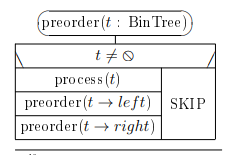
\includegraphics[width=0.3\textwidth]{img/preorder.png}
            \caption{Preorder bejárás}
        \end{figure}
    \item \textit{Inorder}: először bejárja a nulladik részfát, ezután a fa gyökerét dolgozza fel, majd sorban bejárja az 1..r - 1-edik részfákat;
        \begin{figure}[H]
            \centering
            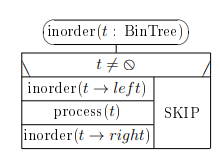
\includegraphics[width=0.3\textwidth]{img/inorder.png}
            \caption{Inorder bejárás}
        \end{figure}
    \item \textit{Postorder}: előbb sorban bejárja a 0..r - 1-edik részfákat, és a fa gyökerét csak a részfák után dolgozza fel
        \begin{figure}[H]
            \centering
            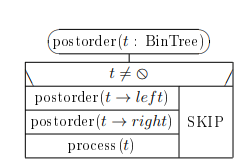
\includegraphics[width=0.3\textwidth]{img/postorder.png}
            \caption{Postorder bejárás}
        \end{figure}
    \item \textit{LevelOrder}: a csúcsokat a gyökértől kezdve szintenként, minden szintet balról jobbra bejárva dolgozza fel.
        \begin{figure}[H]
            \centering
            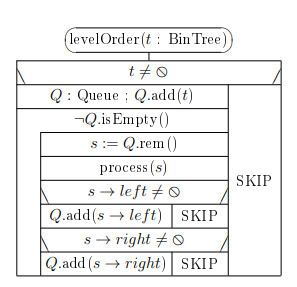
\includegraphics[width=0.3\textwidth]{img/levelOrder.png}
            \caption{LevelOrder bejárás}
        \end{figure}
\end{itemize}

Az első három bejárás tehát nagyon hasonlít egymásra. Nevük megsúgja,
hogy a gyökércsúcsot a részfákhoz képest mikor dolgozzák fel.

\subsection{Ábrázolásaik}
\subsubsection{Grafikus}
A legtermészetesebb és az egyik leggyakrabban használt a bináris fák láncolt
ábrázolása:
\begin{figure}[H]
    \centering
    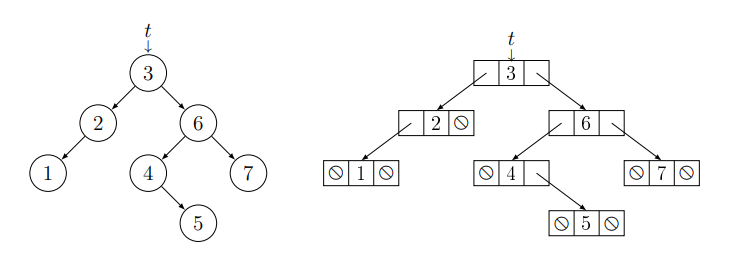
\includegraphics[width=0.6\textwidth]{img/abrazolas.png}
    \caption{Ugyanaz a bináris fa grafikus és láncolt ábrázolással.}
\end{figure}


\subsubsection{Absztrakt}
Az üres fa reprezentációja a $\oslash$  pointer, jelölése tehát ugyanaz, mint az
absztrakt fáknál. A bináris fa csúcsait pl. az alábbi osztály objektumaiként
ábrázolhatjuk, ahol a BinTree absztrakt típus reprezentációja egyszerűen a
Node*.

\begin{figure}[H]
    \centering
    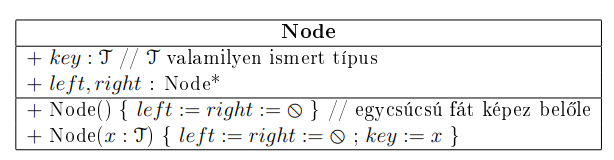
\includegraphics[width=0.5\textwidth]{img/absztrakt_node.png}
\end{figure}

Néha hasznos, ha a csúcsokban van egy parent szülő pointer is, mert a fában
így felfelé is tudunk haladni.
\begin{figure}[H]
    \centering
    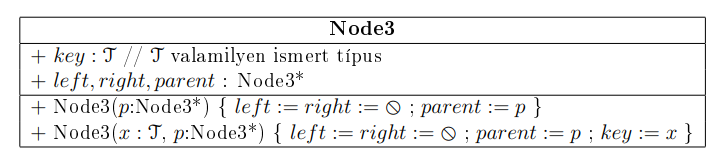
\includegraphics[width=0.5\textwidth]{img/absz_node_parenttel.png}
\end{figure}

\subsubsection{Zárójelezett}

Tetszőleges nemüres bináris fa zárójeles, azaz szöveges alakja:
    ( balRészFa Gyökér jobbRészFa )
Az üres fát az üres string reprezentálja. A könnyebb olvashatóság kedvéért
többféle zárójelpárt is használhatunk. A zárójeles ábrázolás lexikai elemei:
nyitózárójel, csukó zárójel és a csúcsok címkéi.
\begin{figure}[H]
    \centering
    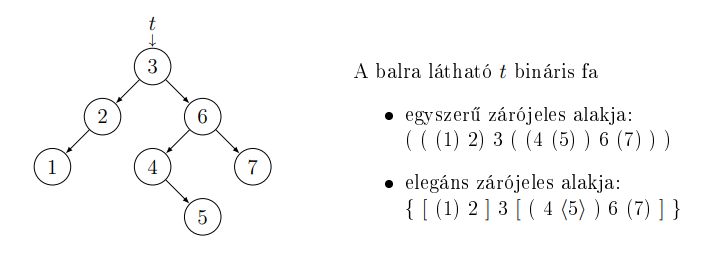
\includegraphics[width=0.5\textwidth]{img/grafikus_szoveges.png}
    \caption{Ugyanaz a bináris fa grafikus és szöveges ábrázolással.}
\end{figure}

\section{Kupac és sor}
A bináris kupac egy konkrét adatszerkezet,
amelyet a prioritásos sor implementálására használnak.
A prioritásos sor általánosabb fogalom, amely többféle adatszerkezetet
vagy algoritmust foglalhat magában a prioritás alapján történő rendezés 
és az elemek elérése szempontjából.

\subsection{Bináris kupac}
Egy teljes bináris fa, 
amelyben az elemek prioritása a csúcsokban található kulcsok alapján van meghatározva. 
A bináris kupac hatékonyan támogatja a prioritásos sor műveleteket,
például az elem beszúrását és eltávolítását a legmagasabb prioritással.
\begin{figure}[H]
    \centering
    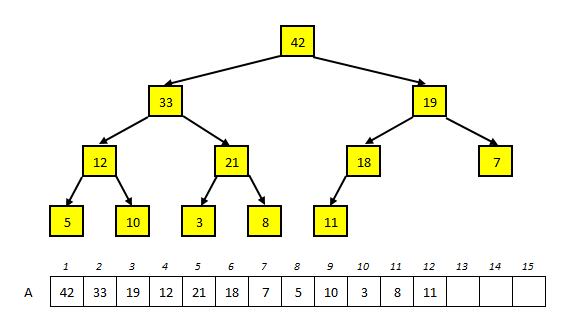
\includegraphics[width=0.5\textwidth]{img/konkret_abrazolas.png}
    \caption{Példa}
\end{figure}

\subsection{Metódusai}
\subsubsection{Hozzáadás}
Új elemet hozzáadunk a kupachoz a levélszintre (a legközelebbi szabad pozícióba).
Ezután a kupacban felfelé haladva összehasonlítjuk az új elemet az ő szülőjével.
Ha az új elem prioritása nagyobb, akkor felcseréljük az elemeket, és folytatjuk a felfelé mozgást a egyel magasabb szintre.
Ezt addig ismételjük, amíg az új elem prioritása nem megfelelő a bináris kupac tulajdonságainak.
\begin{figure}[H]
    \centering
    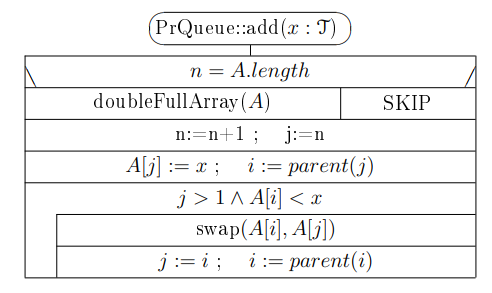
\includegraphics[width=0.5\textwidth]{img/pr_add.png}
    \caption{Az add(x) algoritmusa}
\end{figure}

\subsubsection{Törlés}
A legmagasabb prioritással rendelkező elem mindig a kupac gyökerén található.
Eltávolítjuk(remMax) ezt az elemet, amely a legfelső elem a kupacban.
Ilyenkor a kupac üres lesz, vagy helyettesíteni kell a gyökérlemet az aljában található legutolsó elemmel.
Ha a kupac nem üres, a helyettesítő elemet lefelé mozgatjuk a kupacban, hogy helyreállítsuk a kupac tulajdonságait.
Az elemet összehasonlítjuk a gyermekével, majd a kisebb prioritású gyermekkel cseréljük(sink), ha az nagyobb.
Ezt a folyamatot addig ismételjük, amíg az elem megfelelő helyre nem kerül a kupacban.

\begin{figure}[H]
    \centering
    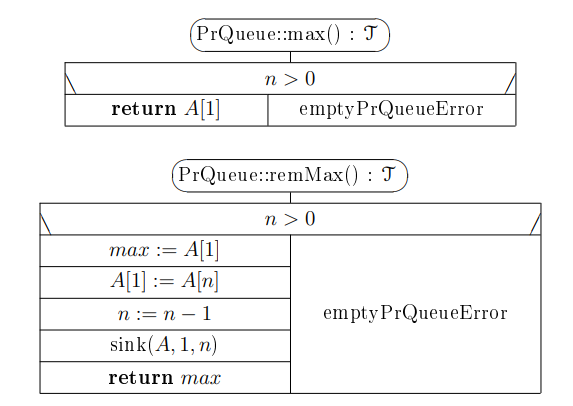
\includegraphics[width=0.4\textwidth]{img/pr_max.png}
    \caption{A remMax() algoritmusa}
\end{figure}

\begin{figure}[H]
    \centering
    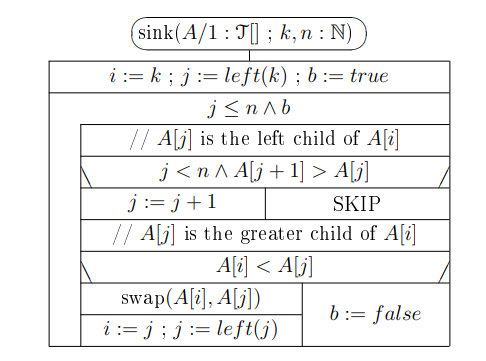
\includegraphics[width=0.4\textwidth]{img/pr_sink.png}
    \caption{A sink(x) algoritmusa}
\end{figure}

\section{Különleges fák}
\subsection{Bináris kereső fa}
\begin{figure}[H]
    \centering
    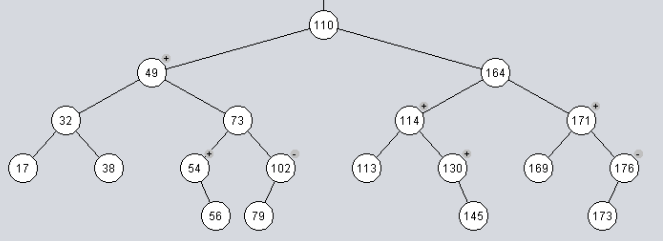
\includegraphics[width=0.5\textwidth]{img/bin_sreach_tree_example.png}
    \caption{Példa bináris kereső fára}
\end{figure}
A bináris kereső fa egy olyan adatszerkezet, amelyet a rendezett adatok hatékony tárolására és lekérdezésére használnak.
\textit{Tulajdonságai}
\begin{itemize}
    \item \textit{Rendezettség}: Minden csúcsnak van egy kulcsa, amelyek alapján eldönthető, hogy a bal részfában (kisebb mint a csúcs) vagy a jobb részfában (nagyobb mint a csúcs) helyezkedik el.
    \item \textit{Gyors keresés}: Lehetővé teszi a gyors keresést a rendezettségnek köszönhetően. Tehát, ha egy elemet keresünk és a csúcstól indulunk egyből tudjuk, hogy jobbra vagy balra van a keresett elem.    
        \begin{figure}[H]
            \centering
            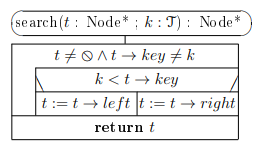
\includegraphics[width=0.4\textwidth]{img/search.png}
            \caption{Keresés bináris kereső fában}
        \end{figure}
    \item \textit{Beszúrás és törlés}: Beszúrásnál az új elemet a megfelelő helyre illesztjük, a rendezettséget figyelembe véve. Törlésnél pedig a struktúrát kell megváltoztatni, hogy a rendezettség megmaradjon.
        \begin{figure}[H]
            \centering
            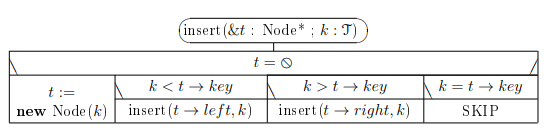
\includegraphics[width=0.4\textwidth]{img/insert.png}
            \caption{Beszúrás bináris kereső fába}
        \end{figure}
        \begin{figure}[H]
            \centering
            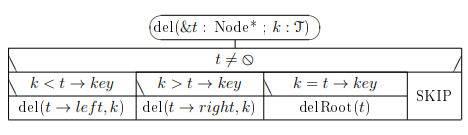
\includegraphics[width=0.4\textwidth]{img/del.png}
            \caption{Törlés bináris kereső fából}
        \end{figure}
    \item \textit{In-order bejárás}: Ezt a bejárást használva, megkapjuk a bináris kereső fa elemeit rendezett sorrendben.
        \begin{figure}[H]
            \centering
            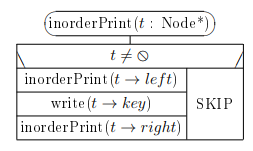
\includegraphics[width=0.4\textwidth]{img/inorder_bin_search_tree.png}
            \caption{In-order bejárás bináris kereső fában}
        \end{figure}
\end{itemize}

\subsection{AVL fa}
Az AVL fa egy speciális bináris kereső fa. Célja az, hogy fenntartsa az egyensúlyt a fa minden csomópontjában,
hogy a keresési, beszúrási és törlési műveletek hatékonyan végezhetők legyenek.
Tehát a bináris kereső fa tulajdonságain felül van még kettő: a magasság és az önkiegyensúlyozás.

\subsubsection{Magasságtulajdonság}
Az AVL fa az egyensúly fenntartása érdekében használja a magasságtulajdonságot. Minden csomópont rendelkezik egy magasságértékkel, amely a csomóponttól a legtávolabbi levél magasságát jelenti. 
Az AVL fában az összes csomópont magasságkülönbsége legfeljebb 1 lehet, vagyis az AVL fa egyensúlyban van.


\subsubsection{Önkiegyensúlyozás}
Ha egy beszúrási vagy törlési művelet után az AVL fa egyensúlyát megsértik, akkor a fa kiegyensúlyozására szolgáló rotációs műveleteket végeznek.
A rotációk célja, hogy a magasságkülönbséget korrigálják és visszaállítsák az AVL fa egyensúlyát.

\subsubsection{Rotációk}
Annak függvényében, hogy melyik oldal változott és mennyire az alábbi rotációkat kell használni.
Ha a bal oldali részfa süllyed egy szintet akkor - jelölést kap, ha a jobb akkor + jelölést.
A ++/-- azt jelenti, hogy az egyik oldalon a részfa magassága kettővel nagyobb mint a másikon.
\begin{figure}[H]
    \centering
    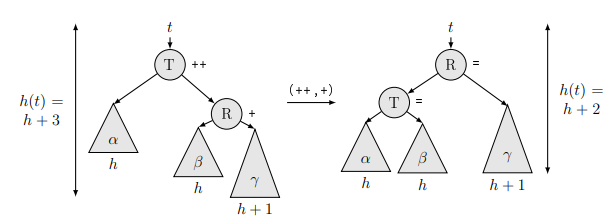
\includegraphics[width=0.5\textwidth]{img/ppp_rotation.png}
    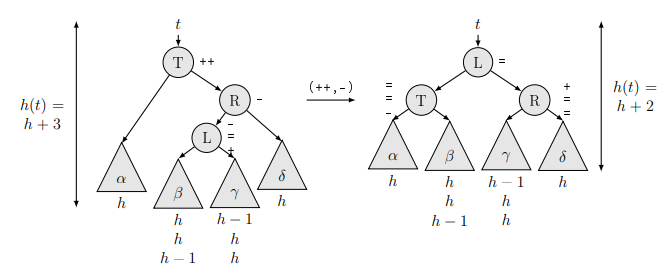
\includegraphics[width=0.5\textwidth]{img/ppm_rotation.png}
    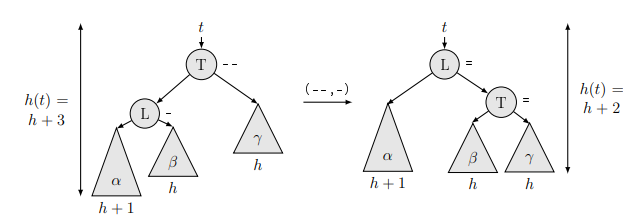
\includegraphics[width=0.5\textwidth]{img/mmm_rotation.png}
    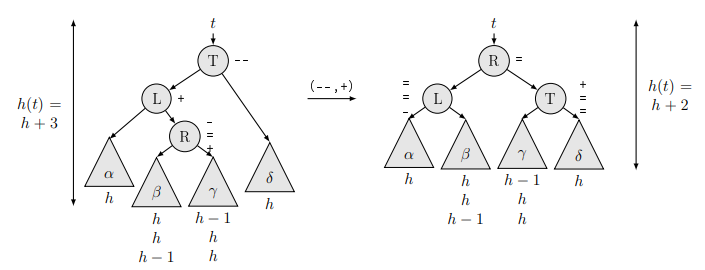
\includegraphics[width=0.5\textwidth]{img/mmp_rotation.png}
    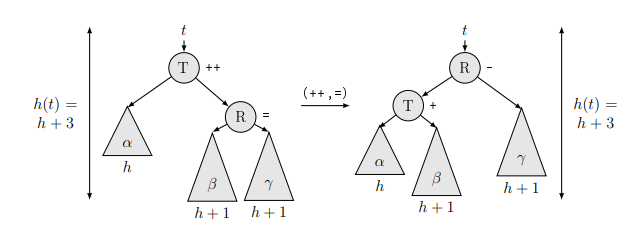
\includegraphics[width=0.5\textwidth]{img/ppn_rotation.png}
    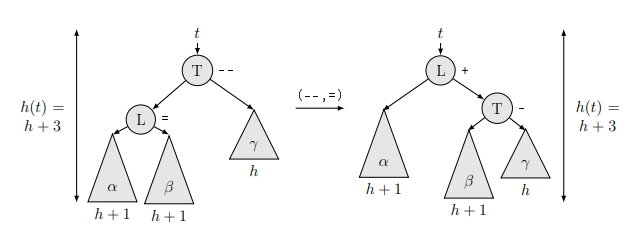
\includegraphics[width=0.5\textwidth]{img/mmn_roatation.png}
\end{figure}

\subsection{B+ fa}
A B+ fa, amiben minden csúcs legfeljebb d mutatót (4 $\leq$  d), és legfeljebb d-1 kulcsot tartalmaz,ahol d a fára jellemző állandó, a B+ fa fokszáma. 
Úgy tekintjük, hogy a belső csúcsokban mindegyikreferencia
két kulcs "között" van, azaz egy olyan részfa gyökerére mutat, amiben minden érték a kétkulcs között található.

\begin{figure}[H]
    \centering
    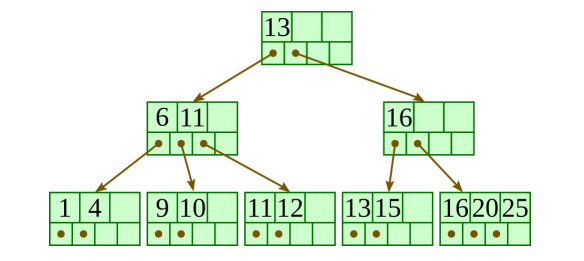
\includegraphics[width=0.5\textwidth]{img/b_plus.png}
    \caption{4-es fokszámú B+ fa}
\end{figure}

Tetszőleges d-ed fokú B+ fa a következő invariánsokat teljesíti, ahol 4 $\leq$ d állandó:
\begin{itemize}
    \item Minden levélben legfeljebb d-1 kulcs, és ugyanennyi, a megfelelő adatrekordrahivatkozó mutató található.
    \item A gyökértől mindegyik levél ugyanolyan távol található.
    \item Minden belső csúcsban eggyel több mutató van, mint kulcs, ahol d a felső határ a mutatók számára.
    \item Minden Cs belső csúcsra, ahol k a Cs csúcsban a kulcsok száma: az első gyerekhez tartozórészfában minden kulcs kisebb, mint a Cs első kulcsa; az utolsó gyerekhez tartozó részfábanminden kulcs nagyobb-egyenlő, mint a Cs utolsó kulcsa; és az i-edik gyerekhez tartozó részfában(2 $\leq$ i $\leq$ k) lévő tetszőleges r kulcsra Cs.kulcs[i-1] $\leq$ r < Cs.kulcs[i].
    \item A gyökércsúcsnak legalább két gyereke van. Kivéve, ha ez a fa egyetlen csúcsa.
    \item Minden, a gyökértől különböző belső csúcsnak legalább d/2 alsó egész-rész gyereke van.
    \item Minden levél legalább d/2 alsó egész-rész kulcsot tartalmaz. A B+ fa által reprezentált adathalmaz minden kulcsa megjelenik valamelyik levélben, balról jobbraszigorúan monoton növekvő sorrendben.
\end{itemize}

\subsubsection{Beszúrás}
Ha a fa üres, hozzunk létre egy új levélcsúcsot, és a beszúrandókulcs/mutató pár a tartalma! 
Különben keressük meg a kulcsnak megfelelő levelet! Ha a levélben márszerepel a kulcs, a beszúrás sikertelen. Egyébként:
\begin{itemize}
    \item Ha a csúcsban van üres hely, szúrjuk be a megfelelő kulcs/mutató párt kulcs szerint rendezetten ebbe a csúcsba!
    \item  Ha a csúcs már tele van, vágjuk szét két csúccsá, középen és osszuk el a d darab kulcsot egyenlően a kétcsúcs között! Ha a létre jött csúcs egy levél, vegyük a létrejött második csúcs legkisebb értékének másolatát, és ismételjük meg ezt a beszúró algoritmust, hogy beszúrjuk azt a szülő csúcsba! Ha a csúcs nemlevél, vegyük ki a középső értéket a kulcsok elosztása során, és ismételjük meg ezt a beszúróalgoritmust, hogy beszúrjuk ezt a középső értéket a szülő csúcsba! (Ha kell, a szülő csúcsot előbblétrehozzuk. Ekkor a B+ fa magassága nő.)
\end{itemize} 

\subsubsection{Törlés}
Keressük meg a törlendő kulcsot tartalmazó levelet! Ha ilyen nincs, a törlés meghiúsul.
\begin{itemize}
    \item Ha keresés során megtalált levélcsúcs egyben a gyökércsúcs is:
    \begin{itemize}
        \item Töröljük a megfelelő kulcsot és a hozzá tartozó mutatót a csúcsból!
        \item Ha a csúcs tartalmaz még kulcsot, kész vagyunk.
        \item Különben töröljük a fa egyetlen csúcsát, és üres fát kapunk.
    \end{itemize}
    \item  A keresés során megtalált levélcsúcs nem a gyökércsúcs:
    \begin{itemize}
        \item Töröljük a megfelelő kulcsot és a hozzá tartozó mutatót a levélcsúcsból!
        \item Ha a levélcsúcs még tartalmaz elég kulcsot és mutatót, hogy teljesítse az invariánsokat, készvagyunk.
        \item Ha a levélcsúcsban már túl kevés kulcs van ahhoz, hogy teljesítse az invariánsokat, de a következő,vagy a megelőző testvérének több van, mint amennyi szükséges, osszuk el a kulcsokat egyenlően közte és a megfelelő testvére között! Írjuk át a két testvér közös szülőjében a két testvérhez tartozóhasító kulcsot a két testvér közül a második minimumára!
        \item Ha a levélcsúcsban már túl kevés kulcs van ahhoz, hogy teljesítse az invariánst, és a következő,valamint a megelőző testvére is a minimumon van, hogy teljesítse az invariánst, akkor egyesítsükegy vele szomszédos testvérével! Ennek során a két testvér közül a (balról jobbra sorrend szerinti)másodikból a kulcsokat és a hozzájuk tartozó mutatókat sorban átmásoljuk az elsőbe, annak eredetikulcsai és mutatói után, majd a második testvért töröljük. Ezután meg kell ismételnünk a törlőalgoritmust a szülőre, hogy eltávolítsuk a szülőből a hasító kulcsot (ami eddig elválasztotta a mostegyesített levélcsúcsokat), a most törölt második testvérre hivatkozó mutatóval együtt. 
    \end{itemize}
    \item Belső — a gyökértől különböző — csúcsból való törlés:
    \begin{itemize}
        \item Töröljük a belső csúcs éppen most egyesített két gyereke közti hasító kulcsot és az egyesítés sorántörölt gyerekére hivatkozó mutatót a belső csúcsból!
        \item Ha a belső csúcsnak van még floor(d/2) gyereke, (hogy teljesítse az invariánsokat) kész vagyunk.
        \item Ha a belső csúcsnak már túl kevés gyereke van ahhoz, hogy teljesítse az invariánsokat, de a következő, vagy a megelőző testvérének több van, mint amennyi szükséges, osszuk el a gyerekeketés a köztük levő hasító kulcsokat egyenlően közte és a megfelelő testvére között, a hasító kulcsokközé a testvérek közti (a közös szülőjükben lévő) hasító kulcsot is beleértve! A gyerekek és ahasító kulcsok újraelosztása során, a középső hasító kulcs a testvérek közös szülőjében a kéttestvérhez tartozó régi hasító kulcs helyére kerül úgy, hogy megfelelően reprezentálja a köztükmegváltozott vágási pontot! (Ha a két testvérben a gyerekek összlétszáma páratlan, akkor azújraelosztás után is annak a testvérnek legyen több gyereke, akinek előtte is több volt!)
        \item Ha a belső csúcsnak már túl kevés gyereke van ahhoz, hogy teljesítse az invariánst, és a következő,valamint a megelőző testvére is a minimumon van, hogy teljesítse az invariánst, akkor egyesítsükegy vele szomszédos testvérével! Az egyesített csúcsot a két testvér közül a (balról jobbra sorrendszerinti) elsőből hozzuk létre. Gyerekei és hasító kulcsai először a saját gyerekei és hasító kulcsaiaz eredeti sorrendben, amiket a két testvér közti (a közös szülőjükben lévő) hasító kulcs követ, ésvégül a második testvér gyerekei és hasító kulcsai jönnek, szintén az eredeti sorrendben. Ezutántöröljük a második testvért. A két testvér egyesítése után meg kell ismételnünk a törlő algoritmusta közös szülőjükre, hogy eltávolítsuk a szülőből a hasító kulcsot
         (ami eddig elválasztotta a mostegyesített testvéreket), a most törölt második testvérre hivatkozó mutatóval együtt.
    \end{itemize}
    \item A gyökércsúcsból való törlés, ha az nem levélcsúcs:
    \begin{itemize}
        \item Töröljük a gyökércsúcs éppen most egyesített két gyereke közti hasító kulcsot és az egyesítés sorántörölt gyerekére hivatkozó mutatót a gyökércsúcsból!
        \item Ha a gyökércsúcsnak van még 2 gyereke, kész vagyunk.
        \item Ha a gyökércsúcsnak csak 1 gyereke maradt, akkor töröljük a gyökércsúcsot, és a megmaradtegyetlen gyereke legyen az új gyökércsúcs! (Ekkor a B+ fa magassága csökken.)    
    \end{itemize}
\end{itemize} 

\section{Hasító táblák}
A hasító tábla (hash table), más néven hasítótábla vagy hash map, egy hatékony adatszerkezet, amely kulcs-érték párokat tárol.
A hasító tábla kulcsokat használ a tárolt értékekhez való gyors hozzáférésre. 
A hasító tábla alapvetően egy tömb, amely az adatokat ún. hash funkció segítségével tárolja és keresi.
\subsection{Hasító függvények}
Amikor egy kulcshoz tartozó értéket hozzá szeretnénk adni a hasító táblához,
először egy hash funkciót alkalmazunk a kulcsra. A hash funkció egy olyan algoritmus, amely egyedi hash kódot generál a kulcs alapján.
A hash kód egy indexet határoz meg a tömbben, ahol az értéket tárolni fogjuk.
\begin{itemize}
    \item \textit{Tárolás:} Az előző lépésben generált hash kód alapján elhelyezzük az értéket a hasító táblában lévő tömb megfelelő indexénél. Ha két vagy több kulcsnak véletlenül ugyanaz a hash kódja, akkor azt hash ütközésnek nevezzük.
    \item \textit{Hash ütközések kezelése:} A hash ütközések kezelése kritikus szerepet játszik a hasító tábla hatékonyságában.
    \begin{itemize}
        \item \textit{Láncolás:} Minden hash kódhoz egy "lánc" tartozik, amely az ütköző kulcsokat tárolja egy adatszerkezetben (általában egy láncolt lista vagy tömb). Ha egy új kulcsnak azonos hash kódja van, a megfelelő láncra kerül, és az érték hozzáadódik a láncolt listához vagy tömbhöz.
        \item \textit{Nyílt címzés:} Az ütköző kulcsokat közvetlenül a tömbben tároljuk, anélkül, hogy külön adatszerkezetet használnánk. Ha egy új kulcsnak ütközik a hash kódja, különböző üres helyeket próbálunk meg keresni a tömbben, amíg üres helyet találunk a tároláshoz.
    \end{itemize}
    \item \textit{Keresés:} A keresés műveletekor ismét alkalmazzuk a hash funkciót a keresett kulcsra, és meghatározzuk az érték tárolásának helyét a hasító táblában. Ha láncolást használunk, akkor végigmegyünk a láncolt listán, hogy a kulcshoz tartozó értéket keresük a hasító táblában, alkalmazzuk a hash funkciót a keresett kulcsra, és meghatározzuk az érték tárolásának helyét a hasító táblában. Ha láncolást használunk, akkor végigmegyünk a láncolt listán vagy a tömbben, és összehasonlítjuk a kulcsokat, hogy megtaláljuk a megfelelő értéket.
    \item \textit{Törlés:} A törlés művelete hasonló a kereséshez. Először alkalmazzuk a hash funkciót a kulcsra, és meghatározzuk az érték tárolásának helyét a hasító táblában. Ha láncolást használunk, akkor végigmegyünk a láncolt listán vagy a tömbben, megtaláljuk a megfelelő értéket, és töröljük azt.
\end{itemize}
A hasító tábla előnyei közé tartozik a gyors adatelérés. Ha a hash funkció jól tervezett és a hash ütközéseket hatékonyan kezeljük, a keresési, beszúrási és törlési műveletek átlagos időkomplexitása O(1) közelíthető, ami nagyon hatékony.
Azonban a hasító tábla néhány korlátot is felvet. Először is, a hash funkció nem mindig garantálja a teljesen egyedi hash kódokat, így lehetőség van a hash ütközések előfordulására. Ezt a megfelelő ütközéskezeléssel kell kezelni. Másodsorban, a hasító tábla fogyasztja a memóriát, különösen, ha nagy méretű tömböt kell tartalmaznia. Az adatmennyiség és a hash funkció hatékonysága közötti egyensúly megtalálása fontos szempont a hatékonyság szempontjából.

\subsection{Próbasorozat}
A próbasorozat egy adatszerkezetekben, például hasító táblákban vagy hasábokban alkalmazott módszer, amelyet a kulcsok egyedi helyét meghatározására használnak.
Amikor egy kulcsot beszúrunk vagy keresünk egy hasító táblában vagy hasábokban, a próbasorozatot használjuk annak meghatározására, hogy hol található a kulcs tárolási helye a táblában.
A próbasorozat olyan sorozat vagy sorrend, amelyet a hash kódhoz vagy a kulcs alapján generálunk.
A leggyakoribb próbasorozatok közé tartoznak:
\begin{itemize}
    \item \textit{Lineáris próbasorozat:} A kiválasztott hash kód vagy index már foglalt a táblában, az algoritmus egymás után következő indexeket próbál meg, amíg üres helyet nem talál. Például, ha az eredeti hash kód 5, és az 5-ös index már foglalt, az algoritmus a 6-os, majd a 7-es indexet próbálja meg, és így tovább.
    \item \textit{Négyzetes próbasorozat:} Az algoritmus négyzet alakban növeli az indexet az ütközés esetén. Például, ha az eredeti hash kód 5, és az 5-ös index már foglalt, az algoritmus a $(5+1^2 = 6)$, majd a $(5+2^2 = 9)$ indexet próbálja meg, és így tovább.
    \item \textit{Dupla hasításos próbasorozat:} Az algoritmus egy második hash funkciót használ az ütközés esetén a következő index meghatározására. A második hash funkció különböző hash kódot generál, amely segít elkerülni az összeomlást és a ciklusokat az indexek között.
\end{itemize}

\section{Gráfok ábrázolásai}
\begin{itemize}
    \item \textit{Szomszédsági mátrix:} A szomszédsági mátrix egy n x n méretű mátrix, ahol n a gráf csúcsainak száma. Az i. sor és j. oszlop eleme az i. és j. csúcs közötti élek jelenlétét vagy súlyát jelzi. Ha az élek irányítottak, akkor a mátrix nem szimmetrikus. Ez a reprezentáció hatékonyan tárolja a gráf szerkezetét, de erőforrásigénye négyzetes arányban nő a csúcsok számával.
    \item \textit{Éllista:} Az éllista egy olyan lista, amely az összes él adatait tartalmazza. Minden élhez tartozik a kezdőcsúcs, a végcsúcs és esetleges további tulajdonságok, például súly. Ez a reprezentáció kevés memóriát igényel, de a gráf szerkezetének lekérdezésekor időigényesebb lehet.
    \item \textit{Szomszédsági lista:} A szomszédsági lista minden csúcshoz tartozó listát tartalmaz, amelyben felsorolják a csúcs közvetlenül szomszédos csúcsait vagy éleit. Ez a reprezentáció általában hatékonyabb a ritka gráfoknál, mivel csak a ténylegesen szomszédos csúcsokat tárolja. Azonban a gráf szerkezetének lekérdezésekor lineáris időigényű lehet.
    \item \textit{Incidencia mátrix:} Az incidencia mátrix egy n x m méretű mátrix, ahol n a csúcsok száma, m pedig az élek száma. Az i. sor és j. oszlop eleme 1, ha az i. csúcs érintett az j. élben, különben 0 vagy más jelölés lehet. Ez a reprezentáció hatékonyan tárolja a gráf szerkezetét és az élek attribútumait, de az erőforrásigénye arányos a csúcsok és élek számával.
\end{itemize}
    

\end{document}